%% This is file `elsarticle-template-3-num.tex',
%%
%% Copyright 2009 Elsevier Ltd
%%
%% This file is part of the 'Elsarticle Bundle'.
%% ---------------------------------------------
%%
%% It may be distributed under the conditions of the LaTeX Project Public
%% License, either version 1.2 of this license or (at your option) any
%% later version.  The latest version of this license is in
%%    http://www.latex-project.org/lppl.txt
%% and version 1.2 or later is part of all distributions of LaTeX
%% version 1999/12/01 or later.
%%
%% The list of all files belonging to the 'Elsarticle Bundle' is
%% given in the file `manifest.txt'.
%%
%% Template article for Elsevier's document class `elsarticle'
%% with numbered style bibliographic references
%%
%% $Id: elsarticle-template-3-num.tex 165 2009-10-08 07:58:10Z rishi $
%% $URL: http://lenova.river-valley.com/svn/elsbst/trunk/elsarticle-template-3-num.tex $
%%
%\documentclass[preprint,12pt]{elsarticle}

%% Use the option review to obtain double line spacing
%% \documentclass[preprint,review,12pt]{elsarticle}

%% Use the options 1p,twocolumn; 3p; 3p,twocolumn; 5p; or 5p,twocolumn
%% for a journal layout:
%% \documentclass[final,1p,times]{elsarticle}
%% \documentclass[final,1p,times,twocolumn]{elsarticle}
%% \documentclass[final,3p,times]{elsarticle}
%% \documentclass[final,3p,times,twocolumn]{elsarticle}
\documentclass[final,5p,times]{elsarticle}
%% \documentclass[final,5p,times,twocolumn]{elsarticle}

%% if you use PostScript figures in your article
%% use the graphics package for simple commands
%% \usepackage{graphics}
%% or use the graphicx package for more complicated commands
\usepackage{graphicx}
%% or use the epsfig package if you prefer to use the old commands
%% \usepackage{epsfig}
\usepackage{subfigure}

%% The amssymb package provides various useful mathematical symbols
\usepackage{amssymb}
%% The amsthm package provides extended theorem environments
%% \usepackage{amsthm}

%% The numcompress package shorten the last page in references.
%% `nodots' option removes dots from firstnames in references.
\usepackage[nodots]{numcompress}

%% The lineno packages adds line numbers. Start line numbering with
%% \begin{linenumbers}, end it with \end{linenumbers}. Or switch it on
%% for the whole article with \linenumbers after \end{frontmatter}.
\usepackage{lineno}

\usepackage[utf8]{inputenc}
\usepackage{caption}

%% Avoids linenumbers to collide with text for 5p format:
\setlength\linenumbersep{3pt}

%% natbib.sty is loaded by default. However, natbib options can be
%% provided with \biboptions{...} command. Following options are
%% valid:

%%   round  -  round parentheses are used (default)
%%   square -  square brackets are used   [option]
%%   curly  -  curly braces are used      {option}
%%   angle  -  angle brackets are used    <option>
%%   semicolon  -  multiple citations separated by semi-colon
%%   colon  - same as semicolon, an earlier confusion
%%   comma  -  separated by comma
%%   numbers-  selects numerical citations
%%   super  -  numerical citations as superscripts
%%   sort   -  sorts multiple citations according to order in ref. list
%%   sort&compress   -  like sort, but also compresses numerical citations
%%   compress - compresses without sorting
%%
%% \biboptions{comma,round}

% \biboptions{}


\journal{Computers \& Graphics}

\begin{document}

\begin{frontmatter}

%% Title, authors and addresses

%% use the tnoteref command within \title for footnotes;
%% use the tnotetext command for the associated footnote;
%% use the fnref command within \author or \address for footnotes;
%% use the fntext command for the associated footnote;
%% use the corref command within \author for corresponding author footnotes;
%% use the cortext command for the associated footnote;
%% use the ead command for the email address,
%% and the form \ead[url] for the home page:
%%
%% \title{Title\tnoteref{label1}}
%% \tnotetext[label1]{}
%% \author{Name\corref{cor1}\fnref{label2}}
%% \ead{email address}
%% \ead[url]{home page}
%% \fntext[label2]{}
%% \cortext[cor1]{}
%% \address{Address\fnref{label3}}
%% \fntext[label3]{}

\title{A Novel GPU-based Sonar Simulation for Real-Time Applications}

%% use optional labels to link authors explicitly to addresses:
%% \author[label1,label2]{<author name>}
%% \address[label1]{<address>}
%% \address[label2]{<address>}
\author[senai,ufba]{Rômulo Cerqueira} \ead{romulo.cerqueira@ufba.br}
\author[senai]{Tiago Trocoli} \ead{trocolit@gmail.com}
\author[senai]{Gustavo Neves}
\author[ufba]{Luciano Oliveira}
\author[senai]{Sylvain Joyeux}
\author[senai,dfki]{Jan Albiez}

\address[senai]{Brazilian Institute of Robotics, SENAI CIMATEC, Salvador, Bahia, Brazil}
\address[ufba]{Intelligent Vision Research Lab, Federal University of Bahia, Salvador, Bahia, Brazil}
\address[dfki]{Robotics Innovation Center, DFKI GmbH, Bremen, Germany}

\begin{abstract}

Sonar simulation requires large computational effort, due the complex physics related on underwater environment, that turn the challenge of reproduce sonar sensor data a non trivial task. However simulating sonar data allows algorithm and control system evaluations with no need to be present in real underwater environment, reducing cost and risks in field experiments, specially, in underwater robotics domain. Based on Graphics Processing Unit (GPU), our work proposes a novel underwater imaging sonar simulator which rely on OpenGL Shading Language (GLSL) chain. Our virtual underwater scene is built on three frameworks, OpenSceneGraph (OSG) reproduces the ocean visual effects, Gazebo deals with physics effects and the Robot Construction Kit (Rock) lets control the sonar on underwater enviroment. Our sonar simulation returns 3-channel matrix as raw data, composed, respectively, by echo intensity, distance to target object and angle distortion information, built around objects shapes and material properties existing in 3D virtual scene. Then, these raw data are treated and after added speckle noise, characteristic sonar noise, to display realistic sonar image. Our evaluation shows the proposed method is capable to operate with high frame rate with good image sonar quality in different virtual underwater scenes.



% Simulating realistic sensor data is of underlying importance to assist the algorithms and control systems evaluation, avoiding the risks and costs of real-life experiments in field robotics. Particularly in underwater robotics domain, this is so due the complexity to reproduce reasonable model of sensors, hydrodynamic forces acting on the robot and environments where the operations take place. This paper introduces an innovative underwater imaging sonar simulator by vertex and fragment processing on GPU (Graphics Processing Unit). The virtual scenario is composed by the integration between Gazebo simulator and the Rock (Robot Construction Kit) framework. The OpenSceneGraph 3D frame is processed during shader rendering in order to compute a 3-channel matrix with depth and intensity buffers and angular distortion values, which is subsequently fused to build the sonar image. Additional characteristics of imaging sonars such as speckle noise, material properties and object's surface irregularities are also addressed and introduced in sonar frame. To export and display simulation resources, this approach was written in C++ with OpenCV support as Rock packages. The method is evaluated by simulating two kind of imaging sonar devices in different scenarios with huge fidelity and high frame rate.

\end{abstract}

\begin{keyword}
%% keywords here, in the form: keyword \sep keyword
Synthetic Sensor Data \sep Sonar Imaging  \sep GPU-based processing \sep Robot Construction Kit (Rock) \sep Underwater Robotics.

\end{keyword}

\end{frontmatter}

%%
%% Start line numbering here if you want
%%
\linenumbers

\section{Introduction}
\label{introduction}

When designing and programming autonomous robotic systems, simulation plays an important role. This applies to physically correct simulations (which are needed to design the hardware but take longer to calculate), as well as to simulations which are not completely physically correct but run in real-time. The latter kind of simulation is important when it comes to developing and testing the control system of autonomous robots, especially the higher level parts. It requires the availability of an applicable simulation platform for rapid prototyping and reproducible virtual environments and sensors to test the decision making algorithms in the control system.

When dealing with autonomous underwater vehicles (AUVs), a real-time simulation plays a key role. Underwater robots usually demand expensive hardware and their target domain can be difficult to access depending on the application. Since an AUV can only scarcely communicate back via mostly unreliable acoustic communication, the robot has to be able to make decisions completely autonomously. While the part dealing with the analysis and interpretation of sensor data can be thoroughly tested on recorded data, for the test and verification of the vehicle's \emph{reaction} to this data, a simulation is needed to reduce the risk of vehicle damage or even vehicle loss in the real world.

Due the AUV acts below the photic zone, with high turbidity and hugh light scattering, the image acquisition by optical devices is limited by short ranges and visibility conditions. Knowing these limitations, the high-frequency sonars systems have been used on navigation and perception applications. Acoustic waves are significantly less affected by water attenuation, facilitating operation at greater ranges even as low to zero visibility conditions with a fast refresh rate. Thus, sonar devices address the main shortcomings of optical sensors though at the expense of providing, in general, noisy data of lower resolution and more difficult interpretation.

In the FlatFish project \cite{albiez2015} was developed an interface to integrate the Gazebo real-time simulator~\footnote{http://gazebosim.org} into the software framework ROCK~\footnote{http://rock-robotics.org/} as presented in \cite{watanabe2015}. With this integration it is able to simulate basic underwater physics and underwater camera systems. The missing part, needed by most underwater robots, was the sonar system.

This paper presents a computationally efficient sonar simulator which manipulates the rendering pipeline to compute a sonar image by two kind of imaging sonar devices.

% ----------------------------------------------------------------------------------

\section{Background}
\label{background}

\subsection{Sonar Image Model}
\label{sonar:model}

Sonars are echo-ranging devices that use acoustic energy to locate and survey objects in a desired area underwater. The sensor's transducer emit pulses of sound wave (or ping) until they hit with any object or be completely absorbed. When the acoustic signal collides with a surface, part of this energy is reflected, while other is refracted. Then the sonar data is built by plotting the echo measured back versus time of acoustic signal.

A single beam transmitted from a sonar is seen in Fig. \ref{fig:sonar_geometry}. The horizontal and vertical beamwidths are represented by the azimuth $\psi$ and elevation $\theta$ angles respectively, where each sampling along the beam is named \textit{bin}. The $x$-axis is perpendicular to the sonar array, the $y$-axis is to the right, $z$-axis points down and the covered area is defined by $r_{min}$ and $r_{max}$. Since the speed of sound underwater is known or can be measured, the time delay between the emitted pulses and their echoes reveals how far the objects are (distance $r$) and how fast they are moving. The backscattered acoustic power in each bin determines the intensity value.

The array of transducer readings, with different azimuth directions, forms the final sonar image. Since all incoming signals converge on the same point, the reflected echoes could have originated anywhere along the corresponding elevation arc at a fixed range, as seen in Fig. \ref{fig:sonar_geometry}. Therefore, the 3D information is lost in the projection into a 2D image \cite{huang2015}.

% ROMULO's COMMENT: IMO the following sentence is a hard afirmation, even with reference.
% According to this operation principle, the projection of a 3D point in the sonar image following a nonlinear model depends on the vertical beamwidth of the point. Approximating this elevation angle to the limit (with zero-elevation plane), leads to a linear model in which the sonar can be represented as an orthographic camera \cite{johannsson2010}.

\begin{figure}[h]
    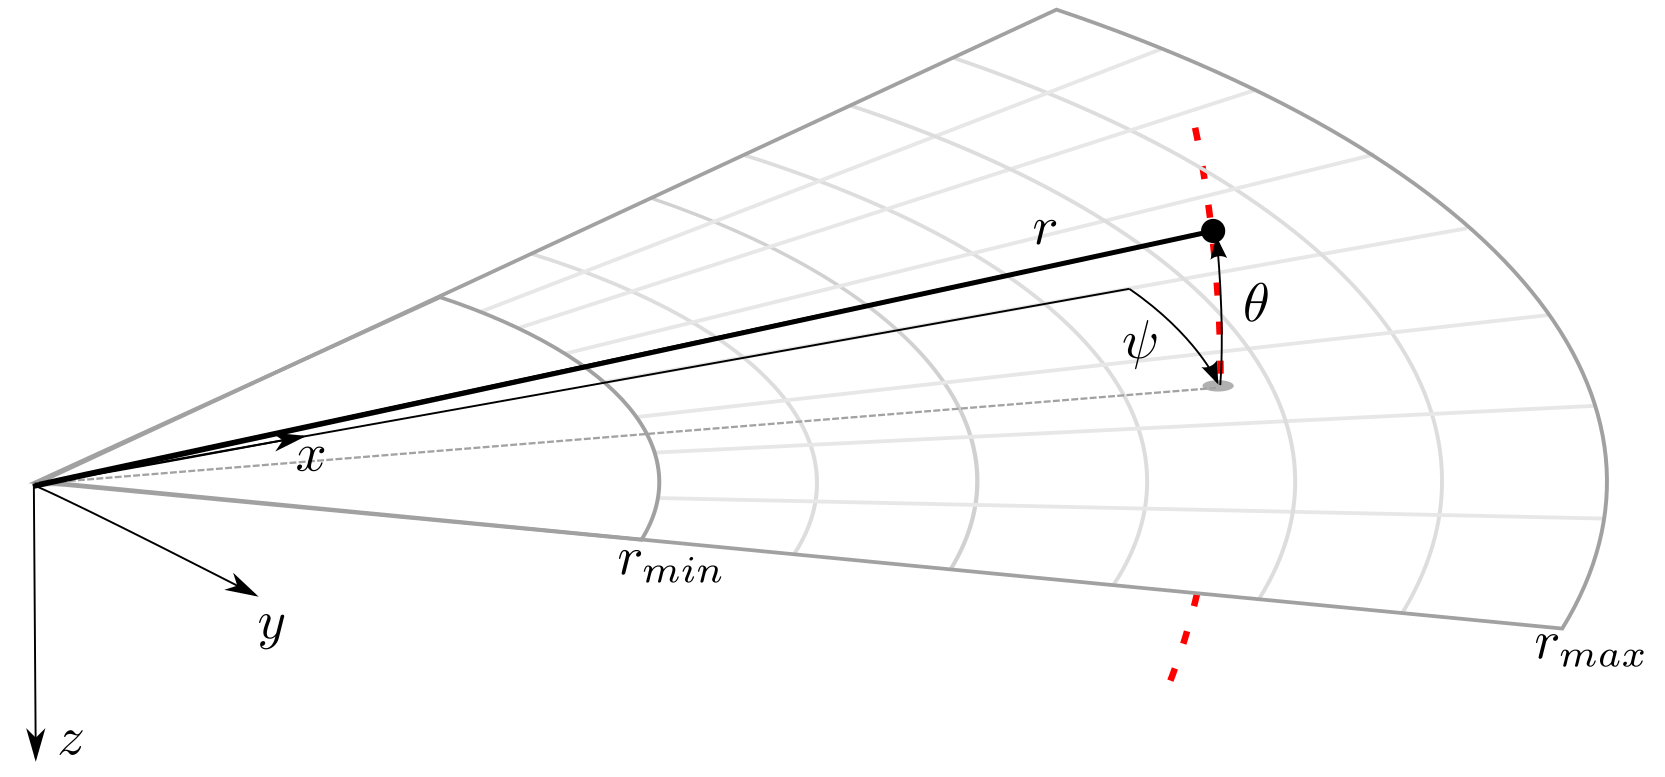
\includegraphics[width=\columnwidth]{figs/sonar_geometry}
    \centering
    \captionsetup{justification=centering}
    \caption{Imaging sonar geometry \cite{huang2015}. By the projection process, all 3D points belong the same elevation arc (represented as dashed red line) will be represented to the same image point in the 2D plane. So the range $r$ and the azimuth angle $\psi$ are measured, however the elevation angle $\theta$ is lost.}
    \label{fig:sonar_geometry}
\end{figure}

% ----------------------------------------------------------------------------------

\subsection{Sonar Characteristics}
\label{sonar:characteristics}

Although the sonar devices address the main shortcomings of optical sensors, they present more difficult data interpretation, such as:

\begin{enumerate}[(a)]
    \item Shadowing: This effect is caused by objects blocking the sound waves transmission and causing regions behind them without acoustic feedback. These regions are defined by a black spot in the image occluding part of the scene;
    \item Non-uniform resolution: The amount of pixels used to represent an intensity record grow as its range increases. This fact causes image distortions and object flatness;
    \item Changes in viewpoint: Imaging the same scene from different viewpoints can cause occlusions, shadows movements and significant alterations of observable objects \cite{hurtos2014}. For instance, when an outstanding object is insonified, its shadow gets shortened as the sonar becomes closer;
    \item Low SNR (Signal-to-Noise Ratio): The sonar suffers from low SNR mainly due the very-long-range scanning and the presence of speckle noise introduced caused by acoustic wave interferences \cite{abbott1973}.
    % \item Inhomogeneous Insonification: Since the water is a loss energy transmission medium, the farthest bins present less intensity than the closest ones.
\end{enumerate}

% ----------------------------------------------------------------------------------

\subsection{Underwater Sonar Devices}
\label{sonar:devices}

The most common types of acoustic sonars are MSIS (Mechanical Scanning Imaging Sonar) and FLS (Forward-Looking Sonar). In the first one (Fig. \ref{fig:swarths:msis}), with one beam per reading, the sonar image is built for each pulse; these images are usually shown on a display pulse by pulse, and the head position reader is rotated according to motor step angle. After a full $360^{\circ}$ sector reading (or the desired sector defined by left and right limit angles), the accumulated sonar data is overwritten. In contrast, the acquisition of a scan image involves a relatively long time and introduces distortions by vehicle movement. This sonar device is useful for obstacle avoidance \cite{ganesan2015} and navigation \cite{ribas2010} applications.

For the FLS, as seen in Fig. \ref{fig:swarths:fls}, with \textit{n} beams being read simultaneously, the whole forward view is scanned and the current data is overwritten by the next one with a high framerate, similar to a streaming video imagery for real-time applications. This imaging sonar is commonly used for navigation \cite{fallon2013}, mosaicing \cite{hurtos2014}, target tracking \cite{liu2016} and 3D reconstruction \cite{huang2015} approaches.

\begin{figure}[h]
    \centering
    \subfigure[][]{
    	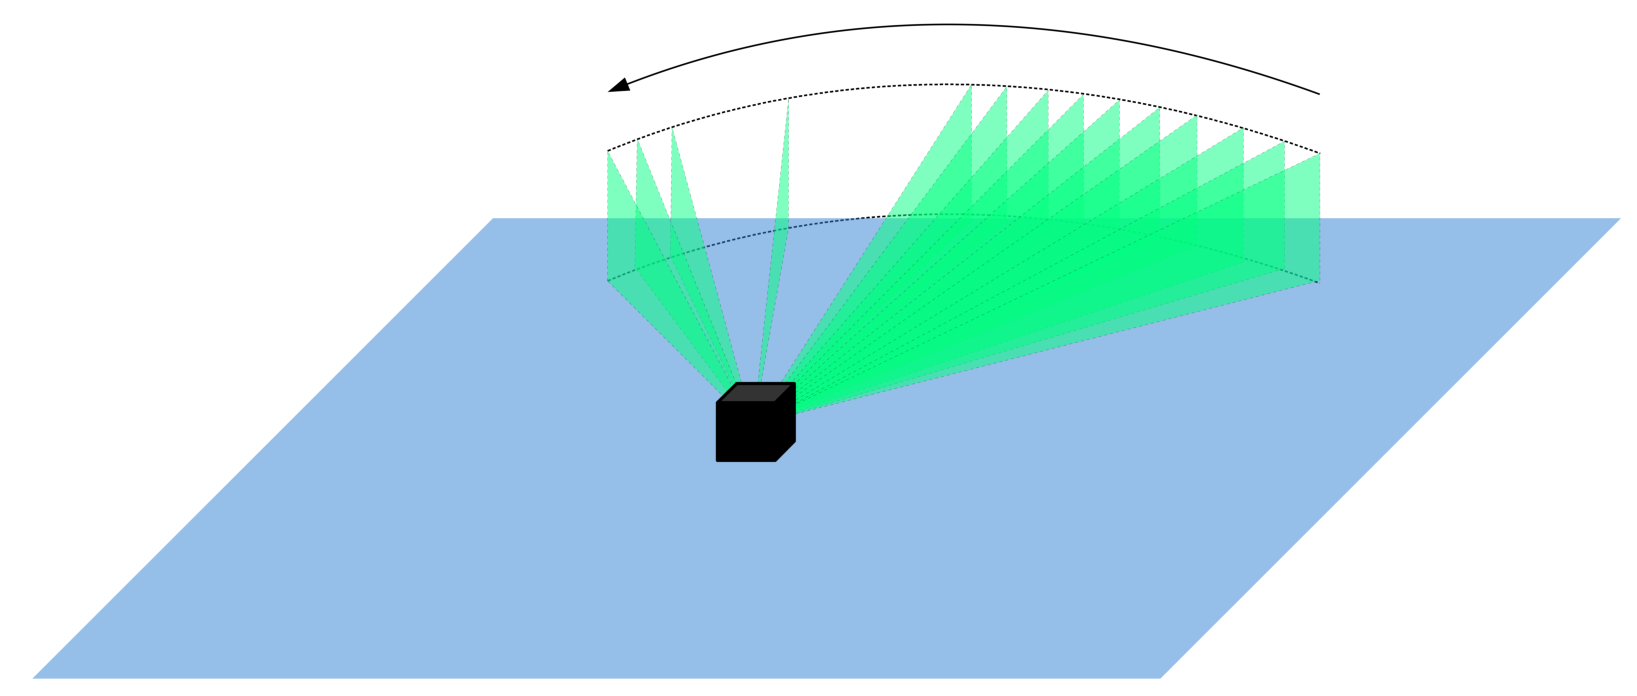
\includegraphics[width=0.95\columnwidth]{figs/sonar_swarths_msis}
        \label{fig:swarths:msis}
    }
    \subfigure[][]{
    	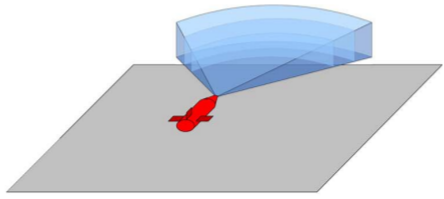
\includegraphics[width=0.95\columnwidth]{figs/sonar_swarths_fls}
        \label{fig:swarths:fls}
    }
    \captionsetup{justification=centering}
    \caption{Different underwater sonar readings: Mechanically Scanning Imaging Sonar \subref{fig:swarths:msis} and Forward-Looking Sonar \subref{fig:swarths:fls}.}
    \label{fig:sonar_devices}
\end{figure}

% ----------------------------------------------------------------------------------

\begin{figure*}[!h]
    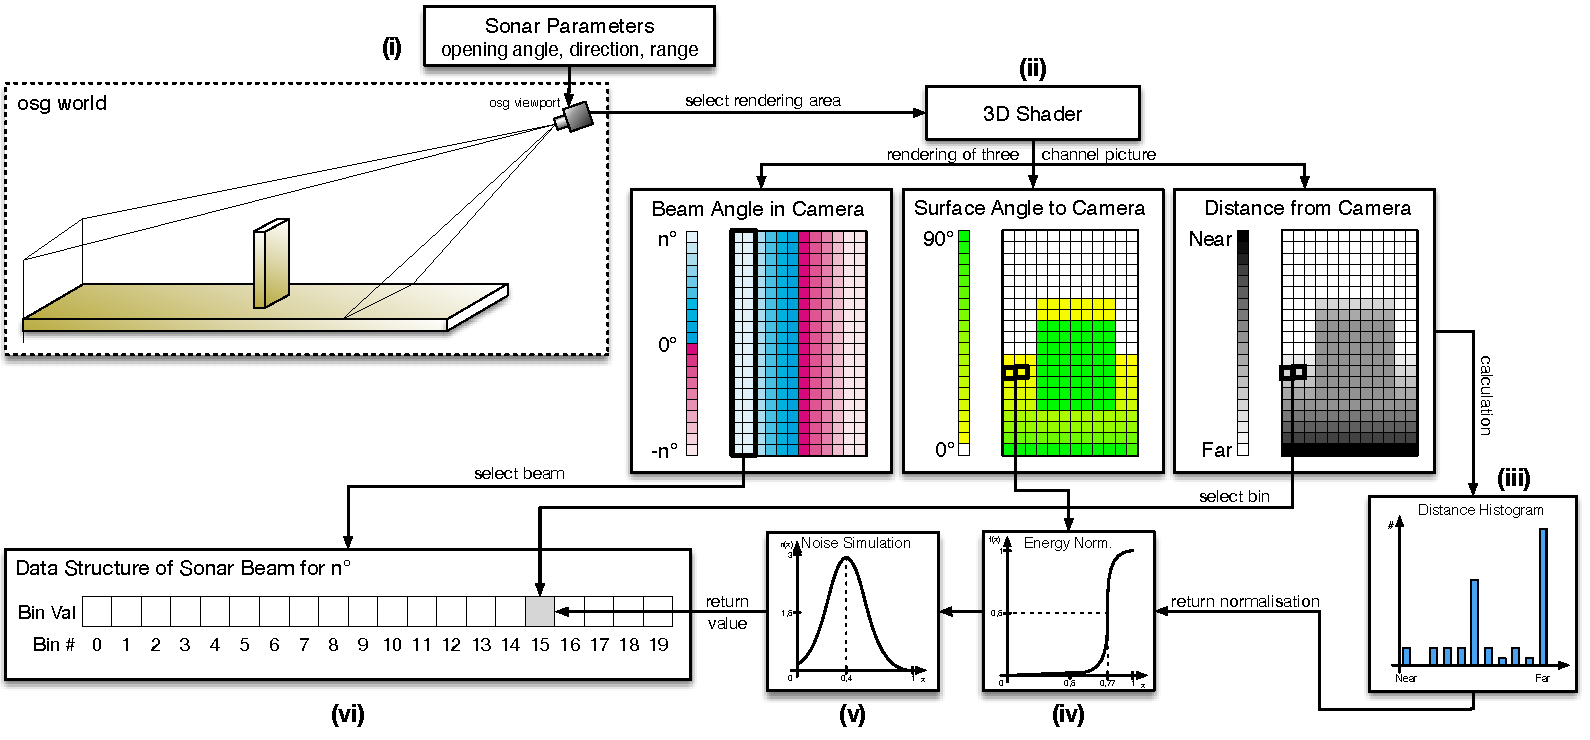
\includegraphics[width=0.85\paperwidth]{figs/sonar_sim}
    \centering
    \captionsetup{justification=centering}
    \caption{A graphical representation of the individual steps to get from the OpenSceneGraph scene to a sonar beam data structure.}
    \label{fig:sonar_sim}
\end{figure*}

\section{Closely-related Works}
\label{relatedworks}

Recent works have been proposed models based on ray tracing and tube tracing techniques to simulate sonar data with very accurate results but at a high computational cost. An application of optical ray tracing to the simulation of underwater side-scan sonar imagery was formulated by Bell \cite{bell1997}. The images were generated by the use of acoustic signals represented by rays. The process of projecting rays is repeated for a 2D-array, representing all angles the sonar can emit signal. Waite \cite{waite2002} used of frequency-domain signal processing to generate synthetic aperture sonar frames. In this method, the acoustic image was created by expressing the Fourier transform of the acoustic pulse used to insonifying the scene.

For FLS simulations, Saç \textit{et al} \cite{sac2015} described the sonar model by computing the ray tracing in frequency domain. When a ray hits an object in 3D space, three parameters are calculated to process the acoustic data: the euclidean distance from the sonar axis, the intensity of returned signal by Lambert Illumination model and the surface normal. The reverberation and shadow phenomena are also addressed. In DeMarco \textit{et al} \cite{demarco2015}, the rays are used in Gazebo and ROS~\footnote{http://www.ros.org/}(Robot Operating System) integration to simulate the acoustic pulse and produce a 3D point cloud of covered area. Since the material reflectivity was statically defined, it resulted in the same intensity values for all points on a single object. Gu \textit{et al} \cite{gu2013} modeled a FLS device where the ultrasound beams were formed by a set of rays. However, the acoustic image is significantly limited by its representation by only two colors: white, when the ray strike an object, and black for shadow areas. This approach was evolved by Kwak et al \cite{kwak2015} by adding a sound pressure attenuation to produce the gray-scale sonar frame, while the other physical characteristics related to sound transmission are disregarded.

The proposed approach herein entails several novelties. As opposed to the related works, the depth and normal values are directly manipulated during the scene formation, which generate sonar frames with a low computational cost and allow the usage by real-time applications. Also, this method is able to reproduce any type of underwater sonar images, as seen in evaluation tests with two kind of sonar devices.

In addition to our previous work \cite{cerqueira2016}, the normal data can also be defined by bump mapping technique and material's reflectivity. Moreover, the speckle noise is modeled as a non-uniform Gaussian distribution and added to final sonar image.

% ----------------------------------------------------------------------------------

\section{GPU-based Sonar Simulation}
\label{dev}

The goal of this work is to simulate any kind of underwater sonar by vertex and fragment processing, with a low computational-time cost. The complete pipeline of this implementation, from the virtual scene to the synthetic acoustic image, is seen in Fig. \ref{fig:sonar_sim} and is detailed in the following subsections. The sonar simulation is written in C++ with OpenCV~\footnote{http://opencv.org/} support as Rock packages.

% ----------------------------------------------------------------------------------

\subsection{Underwater Environment}
\label{dev:uwscene}

The Rock-Gazebo integration \cite{watanabe2015} provides the underwater scenario and allows real-time Hardware-in-the-Loop simulations, where Gazebo handles the physical engines and the Rock's visualization tools are responsible by the scene rendering. The graphical data in Rock are based on OpenSceneGraph~\footnote{http://www.openscenegraph.org/} library, an open source C/C++ 3D graphics toolkit built on OpenGL. The osgOcean~\footnote{http://wiki.ros.org/osgOcean} library is used to simulate the ocean's visual effects, and the ocean buoyancy is defined by the Gazebo plugin as described in Watanabe et al \cite{watanabe2015}.

All scene's aspects, such as world model, robot parts (including sensors and joints) and others objects presented in the environment are defined by SDF files, which uses the SDFormat~\footnote{http://sdformat.org}, a XML format used to describe simulated models and environments for Gazebo. Also, the vehicle and sensor robot description must contain a geometry file. Visual geometries used by the rendering engine are provided in COLLADA format and the collision geometries in STL data.

Each component described in the SDF file becomes a Rock component, which is based on the Orocos RTT (Real Time Toolkit)~\footnote{http://www.orocos.org/rtt} and provides ports, properties and operations as its communication layer. When the models are loaded, Rock-Gazebo creates ports to allow other system components to interact with the simulated models \cite{cerqueira2016}. A resulting scene sample of this integration is seen in Fig. \ref{fig:uwscene}.

\begin{figure}[!h]
    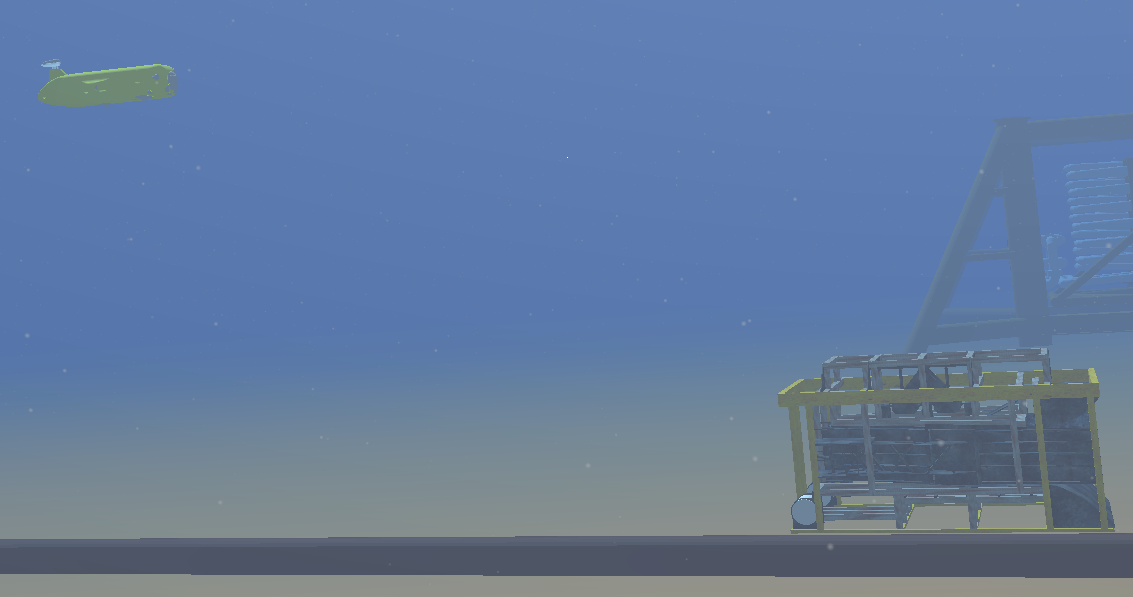
\includegraphics[width=\columnwidth]{figs/uwscene2}
    \centering
    \captionsetup{justification=centering}
    \caption{FlatFish AUV in ROCK-Gazebo underwater scene.}
    \label{fig:uwscene}
\end{figure}

% ----------------------------------------------------------------------------------

\subsection{Shader Rendering}
\label{dev:shader}

Modern graphics hardware presents programmable tasks embedded in GPU. Based on parallel computing, this approach can speed up 3D graphics processing and reduce the computational effort of Central Processing Unit (CPU).

The rendering pipeline can be customized by defining programs on GPU called shaders. A shader is written in OpenGL Shading Language (GLSL)~\footnote{https://www.opengl.org/documentation/glsl/}, a high-level language with a C-based syntax which enables more direct control of graphics pipeline avoiding the usage of low-level or hardware-specific languages. Shaders can describe the characteristics of either a vertex or a fragment (a single pixel). Vertex shaders are responsible by transform the vertex position into a screen position by the rasterizer, generating texture coordinates for texturing, and lighting the vertex to determine its color. The rasterization results in a set of pixels to be processed by fragment shaders, which manipulate their locations, depth and alpha values and interpolated parameters from the previous stages, such as colors and textures \cite{fernando2003}.

In this work, the underwater scene is sampled by a virtual camera, whose optical axis is aligned with the intended viewing direction of the imaging sonar, as well as the covered range and opening angle. By programming the fragment and vertex shaders, the sonar data is computed as:

\begin{itemize}[(a)]
    \item \textit{Depth} is the camera focal length and is calculated by the euclidean distance to object's surface point;
    \item \textit{Intensity} presents the echo reflection energy based on object's surface normal angle to the camera;
    \item \textit{Angular distortion} is the angle formed from the camera center column to the camera boundary column, for both directions.
\end{itemize}

These data are normalized in [0,1] interval, where means no energy and maximum echo energy for intensity data respectively. For depth data, the minimum value portrays a close object while the maximum value represents a far one, limited by the sonar maximum range. Angle distortion value is zero in image center column which increases for both borders to present the half value of horizontal field of view.

Most real-world surfaces present irregularities and different reflectances. For more realistic sensing, the normal data can also be defined by bump mapping and material properties. Bump mapping is a perturbation rendering technique to simulate wrinkles on the object's surface by passing textures and modifying the normal directions on shaders. It is much faster and consumes less resources for the same level of detail compared to displacement mapping, because the geometry remains unchanged. Since bump maps are built in tangent space, interpolating the normal vertex and the texture, a TBN (Tangent, Bitangent and Normal) matrix is computed to convert the normal values to world space. The different scenes representation is seen in Fig. \ref{fig:sonar_bump_mapping}.

\begin{figure*}[!h]
    \centering
    \subfigure[][]{
        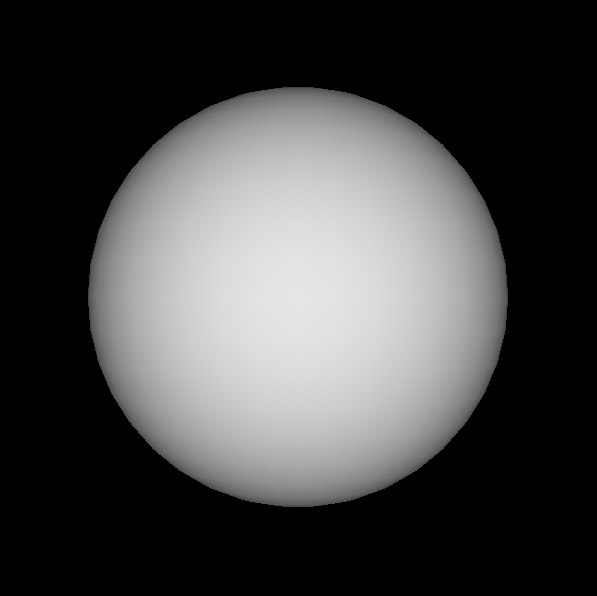
\includegraphics[width=0.27\paperwidth]{figs/bump_0}
        \label{fig:bump_0}
    }
    \subfigure[][]{
        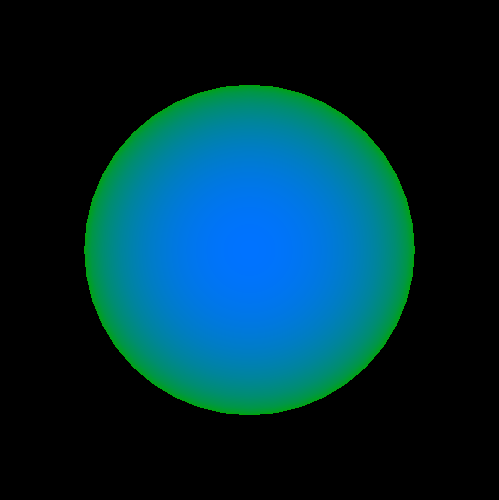
\includegraphics[width=0.27\paperwidth]{figs/bump_1}
        \label{fig:bump_1}
    }
    \subfigure[][]{
        
\includegraphics[width=0.27\paperwidth]{figs/bump_2}
        \label{fig:bump_2}
    }
    \subfigure[][]{
        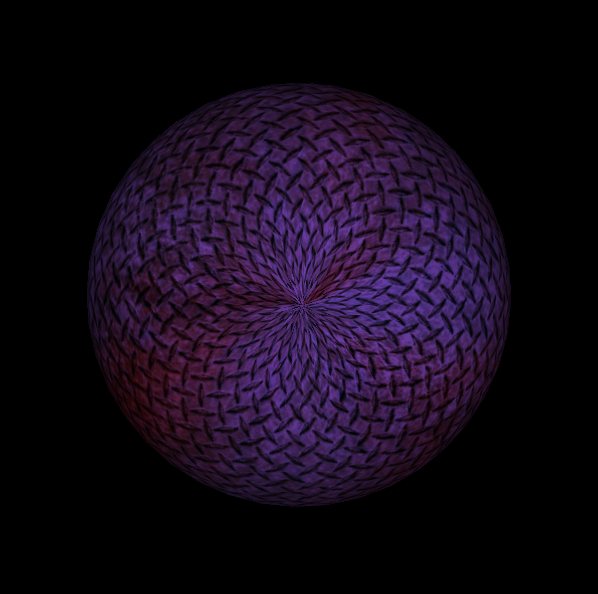
\includegraphics[width=0.27\paperwidth]{figs/bump_3}
        \label{fig:bump_3}
    }
    \subfigure[][]{
        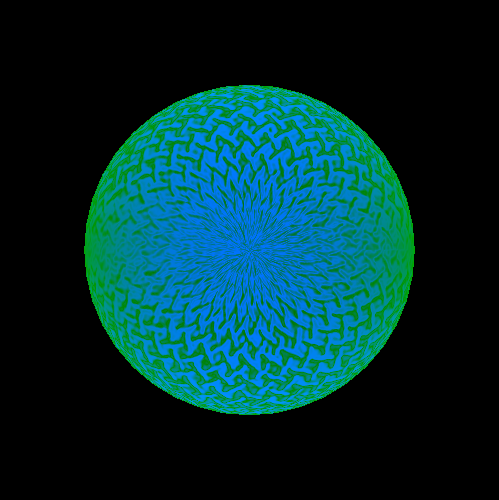
\includegraphics[width=0.27\paperwidth]{figs/bump_4}
        \label{fig:bump_4}
    }
    \subfigure[][]{
        
\includegraphics[width=0.27\paperwidth]{figs/bump_5}
        \label{fig:bump_5}
    }
    \captionsetup{justification=centering}
    \caption{Shader rendering with bump mapping processing example: sphere without texture \subref{fig:bump_0} and with texture \subref{fig:bump_3}; their respective shader image representation in \subref{fig:bump_1} and \subref{fig:bump_4}, where the blue is the normal channel and green is the depth one; and the final acoustic image in \subref{fig:bump_2} and \subref{fig:bump_5}. By bump mapping technique, the texture changes the normal directions and the sonar image are more realistic in comparison to real objects appearances.}
    \label{fig:sonar_bump_mapping}
\end{figure*}

Moreover, the reflectance allows to describe properly the intensity back from observable objects in shader processing according their material properties (e.g. aluminium has more reflectance than wood and plastic). When an object has its reflectivity defined, the reflectance value $R$ is passed to fragment shader and must be positive. As seen in Fig. \ref{fig:sonar_reflectances}, when the normal values are directly proportional to the reflectance value $R$.

\begin{figure}[h]
    \centering
    \subfigure[][]{
    	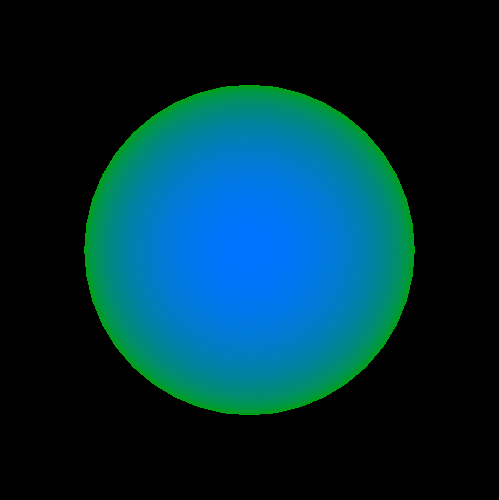
\includegraphics[width=0.47\columnwidth]{figs/reflectance_0}
        \label{fig:reflectance:0}
    }
    \subfigure[][]{
    	
\includegraphics[width=0.47\columnwidth]{figs/reflectance_0_35}
        \label{fig:reflectance:0.35}
    }
    \subfigure[][]{
    	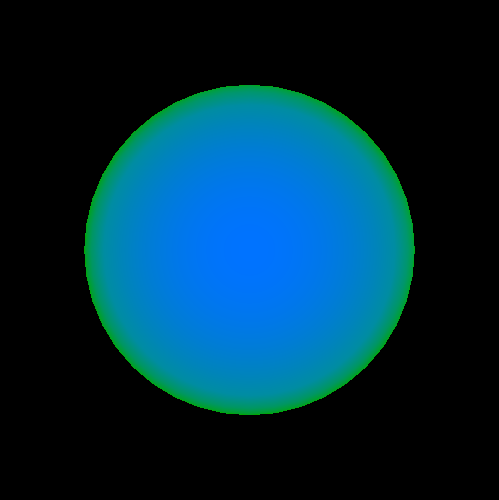
\includegraphics[width=0.47\columnwidth]{figs/reflectance_1_40}
        \label{fig:reflectance:1.40}
    }
    \subfigure[][]{
    	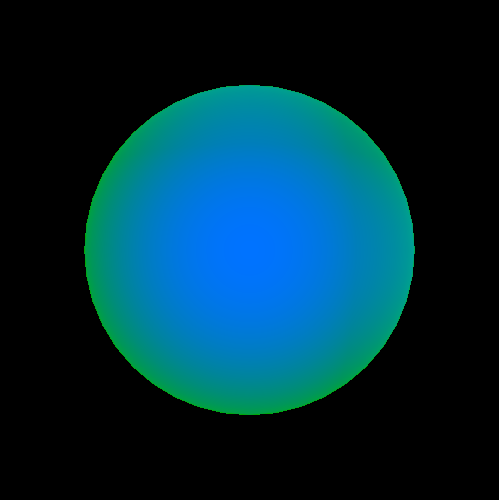
\includegraphics[width=0.47\columnwidth]{figs/reflectance_2_12}
        \label{fig:reflectance:2.12}
    }
    \captionsetup{justification=centering}
    \caption{Examples of different reflectance values $R$ on shader image representation, where blue is the normal channel and green is the depth channel: raw image \subref{fig:reflectance:0}; $R = 0.35$ \subref{fig:reflectance:0.35}; $R = 1.40$ \subref{fig:reflectance:1.40}; and $R = 2.12$ \subref{fig:reflectance:2.12}.}
    \label{fig:sonar_reflectances}
\end{figure}

At the end, the shader process gives a 3-channel matrix data of intensity, depth and angular distortion stored in each channel.

% ----------------------------------------------------------------------------------

\subsection{Synthetic Sonar Data}
\label{dev:sonardata}

The 3D shader matrix is processed in order to build the corresponding acoustic representation. Since the angular distortion is radially spaced over the horizontal field of view, where all pixels in the same column have the same angle value, the first step is to split the image in number of beam parts. Each column is correlated with its respective beam, according to sonar bearings, as seen in Fig. \ref{fig:sonar_sim}.

Each beam subimage is converted into bin intensities using the depth and intensity channels. In a real imaging sonar, the echo measured back is sampled over time and the bin number is proportional to sensor's range. In other words, the initial bins represent the closest distances, while the latest bins are the furthest ones. Therefore, a distance histogram is evaluated to group the subimage pixels with their respective bins, according to depth channel. This information is used to calculate the accumulated intensity of each bin.

Due to acoustic beam spreading and absorption in the water, the final bins have less echo strength than the first ones, because the energy is lost two-way in the environment. In order to solve this, the sonar devices use a energy normalization based on time-varying gain for range dependence compensation which spread losses in the bins \cite{urick2013}. In this simulation approach, the accumulated intensity in each bin is normalized as

\begin{equation}
    \label{eq:1}
    I_{bin} = \sum\limits_{x=1}^N \frac{1}{N} \times S(i_{x}) \, ,
\end{equation}

where $I_{bin}$ is the intensity in the bin after the energy normalization, $x$ is the pixel in the shader matrix, $N$ is the depth histogram value (number of pixels) of that bin, $S(i_{x})$ is the sigmoid function and $i_{x}$ is the intensity value of the pixel $x$.

Finally, the sonar image resolution needs to be big enough to fill all bins informations. In this case, the number of bins involved is in direct proportion to the sonar image resolution.

% ----------------------------------------------------------------------------------

\subsection{Noise Model}
\label{dev:noise}

Imaging sonar systems are perturbed by a multiplicative noise known as speckle. It is caused by coherent processing of backscattered signals from multiple distributed targets, that degrades image quality and the visual evaluation. Speckle noise results in constructive and destructive interferences which are shown as bright and dark dots in the image. The noisy image has been expressed as \cite{lee1980}:

\begin{equation}
\label{eq:2}
y(t) = x(t) \times n(t) \, ,
\end{equation}

where $t$ is the time instant, $y(t)$ is the noised image, $x(t)$ is the free-noise image and $n(t)$ is the speckle noise matrix.

This kind of noise is well-modeled as a Gaussian distribution. The physical explanation is provided by the Central Limit of Theorem, which states that the sum of many independent and identically distributed random variables tends to behave a Gaussian random variable \cite{papoulis2002}.

A Gaussian distribution is built following a non-uniform distribution, skewed towards low values, as seen in Fig. \ref{fig:sonar_sim}, and applied as speckle noise in the simulated sonar image. After that, the simulation sonar data process is done.

\subsection{Rock's Sonar Structure}
\label{dev:rock}

To export and display the sonar image, the simulated data is encapsulated as Rock's sonar data type and provided as an output port of Rock's component.

% ----------------------------------------------------------------------------------

\section{Results and Discussion}
\label{results}

\subsection{Experiment Settings}

For the evaluation of the proposed simulator, the experiments were conducted by using a 3D model of FlatFish AUV equipped with two MSIS and one FLS sensors on different scenarios. The MSIS sensors are located in AUV's top and back and they are configured as follows: opening angle of $3^{\circ}$ by $35^{\circ}$, 500 bins in the single beam, a full $360^{\circ}$ sector scan reading and a motor step of $1.8^{\circ}$. By other hand, the FLS takes place in AUV's bottom with the following set: field of view of $120^{\circ}$ by $20^{\circ}$, 256 beams simultaneously, 1000 bins per each beam and angle tilt between the sonar and AUV of $20^{\circ}$. While the scene's frames were captured by the sonars, we sequentially present the resulting simulated acoustic images.

\subsection{Experimental Evaluation}

The virtual FLS from FlatFish AUV was used to insonify scenes in three scenarios. A docking station, in parallel with a pipeline on the seabed, composes the first scenario, as seen in Fig. \ref{fig:fls_scene1}. The target's surface is well-defined in the simulated acoustic frame, as seen in Fig. \ref{fig:fls_sim1}, even as the shadows and speckle noise. Given the docking station is metal-made, the texture and reflectivity were set, resulting in a higher intensity shape in comparison with the other targets.

The second scenario presents the vehicle in front of a manifold model on a non-uniform seabed, as seen in Fig. \ref{fig:fls_scene2}. The target model was insonified to generate the sonar frame from the underwater scene. The frontal face of the target, as well the portion of the seabed and the degraded data by noise, are clearly visible in the FLS image. Also, a long acoustic shadow is formed behind the manifold, occluding part of the scene.

The third scenario contains a SSIV (SubSea Isolation Valve) structure connected with a pipeline in the bottom, presented in Fig. \ref{fig:fls_scene3}. The targets' shapes are well-defined, such as their shadows.

Due the sensor configuration and the robot position, the initial bins usually present a blind region in the three simulated scenes, caused by absence of objects at lower ranges, similar with real images. Also, the brightness of seafloor decreases when it makes farthest from sonar due the normal orientation of surface.

\begin{figure*}[!h]
    \centering
    \subfigure[][]{
        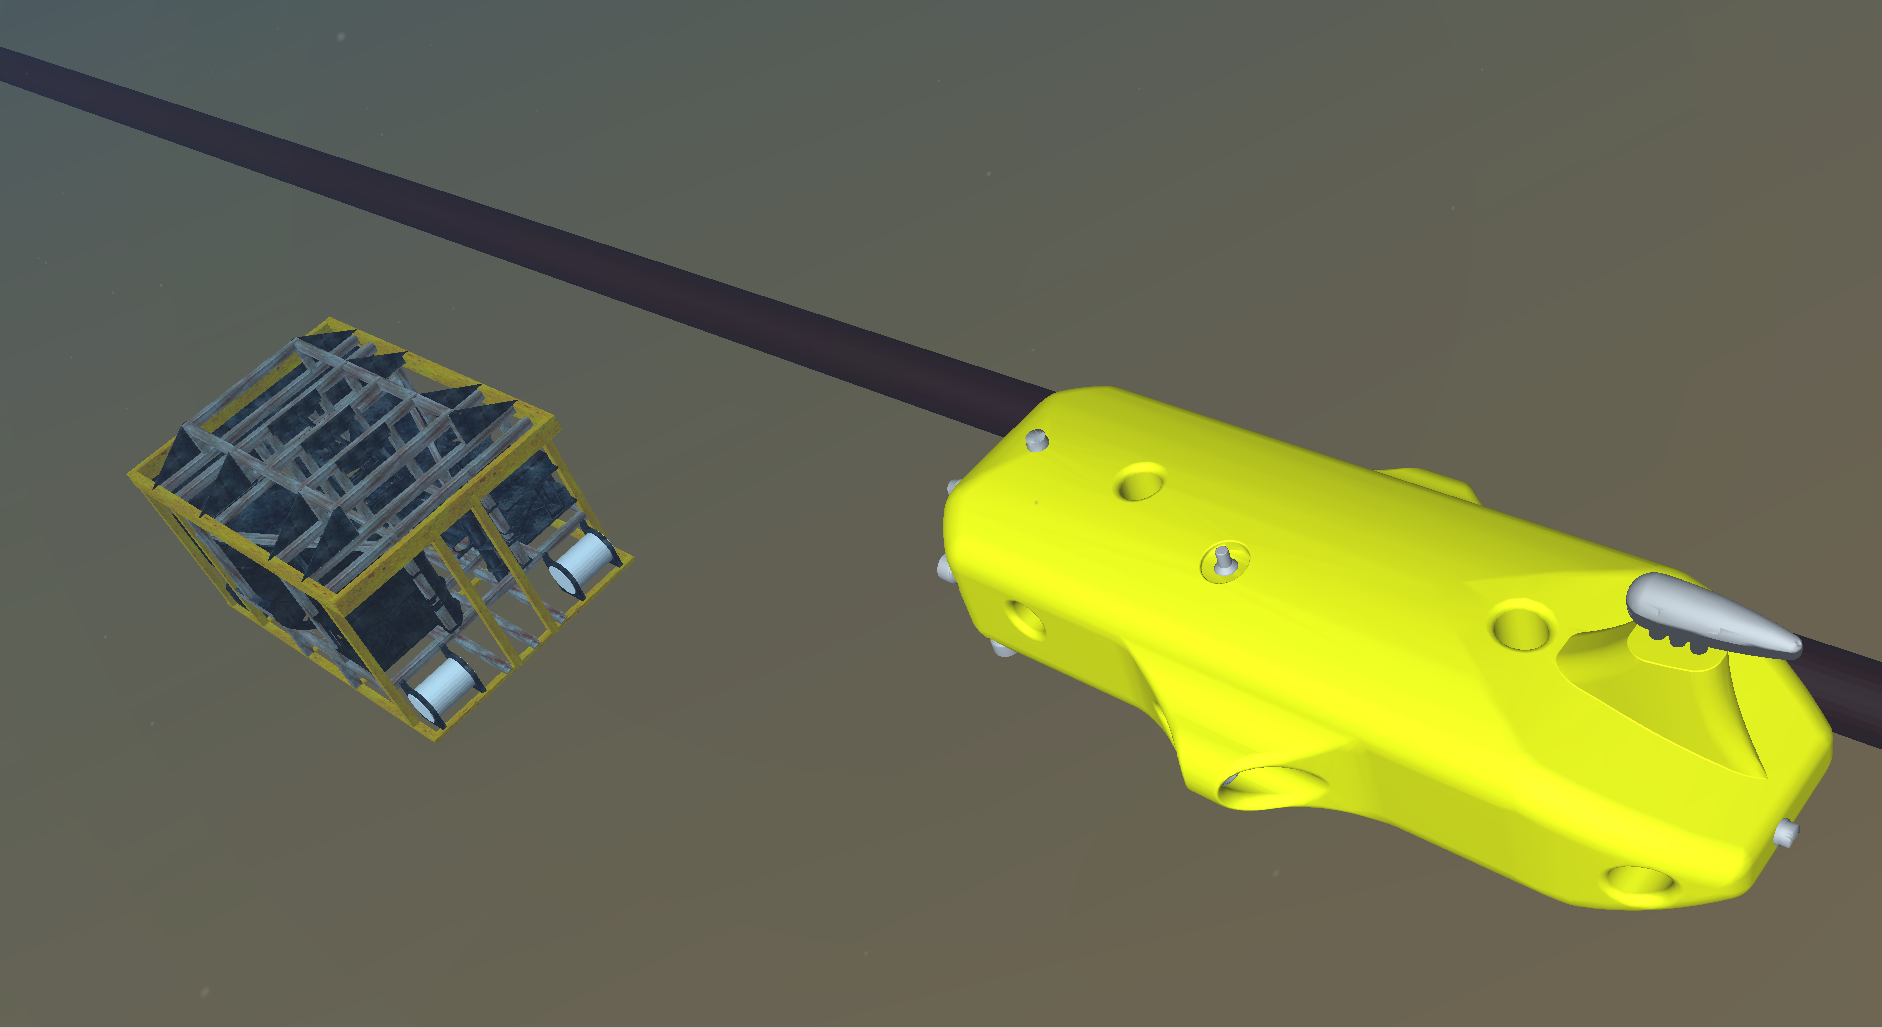
\includegraphics[width=0.425\paperwidth,height=6cm]{figs/fls_scene1}
        \label{fig:fls_scene1}
    }
    \subfigure[][]{
        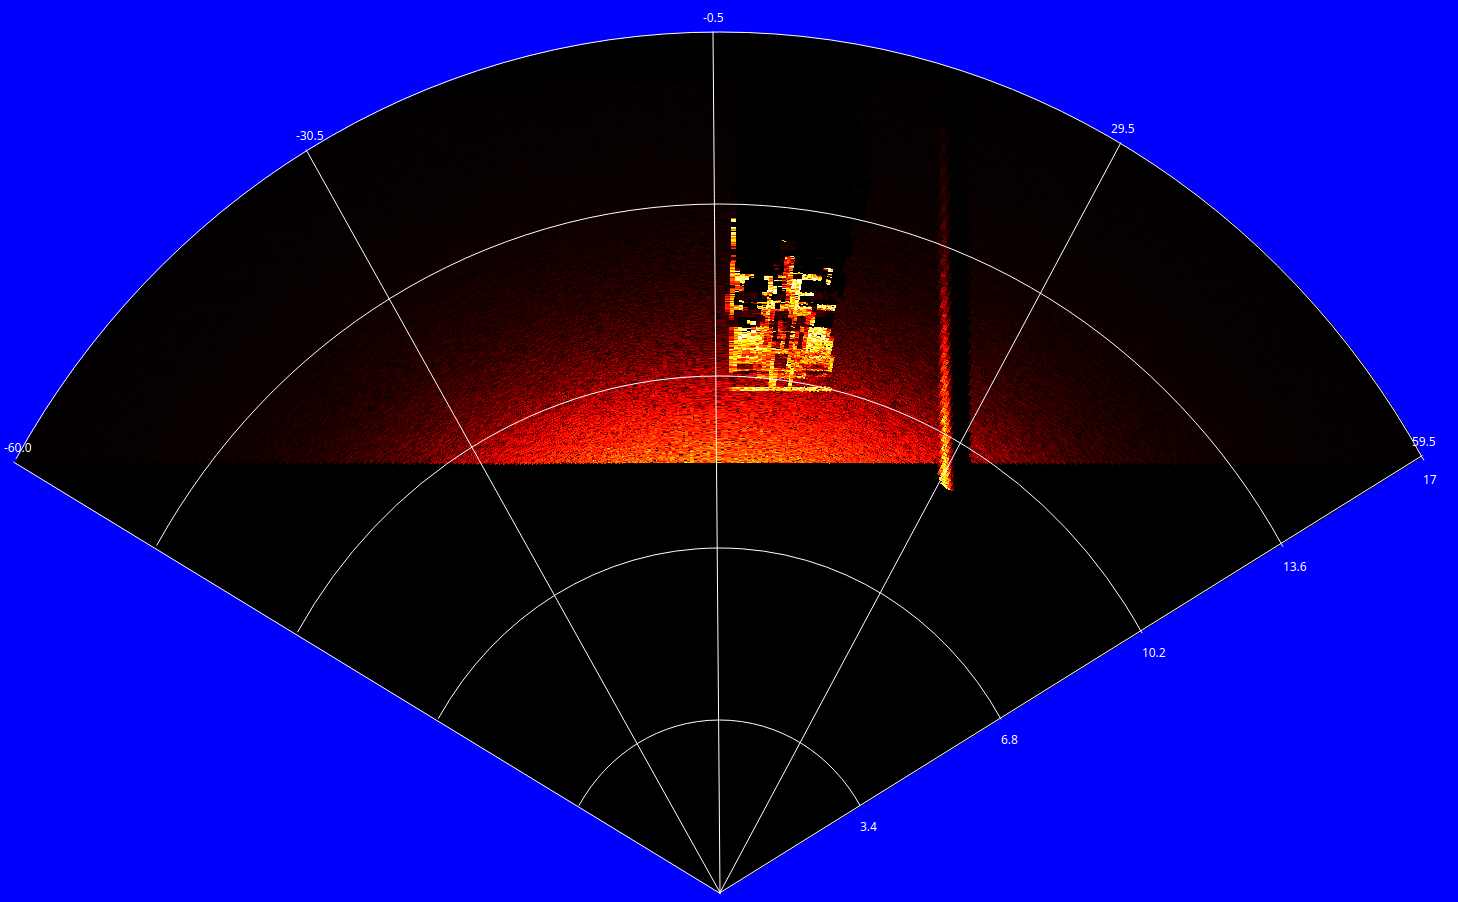
\includegraphics[width=0.425\paperwidth,height=6cm]{figs/fls_sim1}
        \label{fig:fls_sim1}
    }
    \subfigure[][]{
        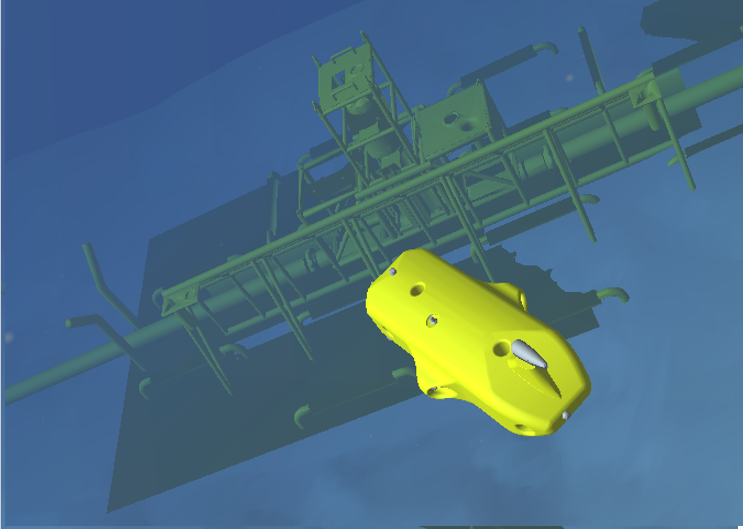
\includegraphics[width=0.425\paperwidth,height=6cm]{figs/fls_scene2}
        \label{fig:fls_scene2}
    }
    \subfigure[][]{
        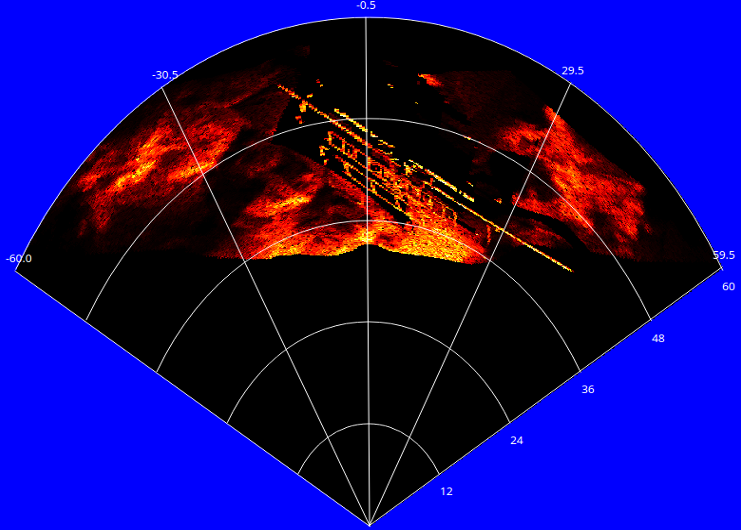
\includegraphics[width=0.425\paperwidth,height=6cm]{figs/fls_sim2}
        \label{fig:fls_sim2}
    }
    \subfigure[][]{
        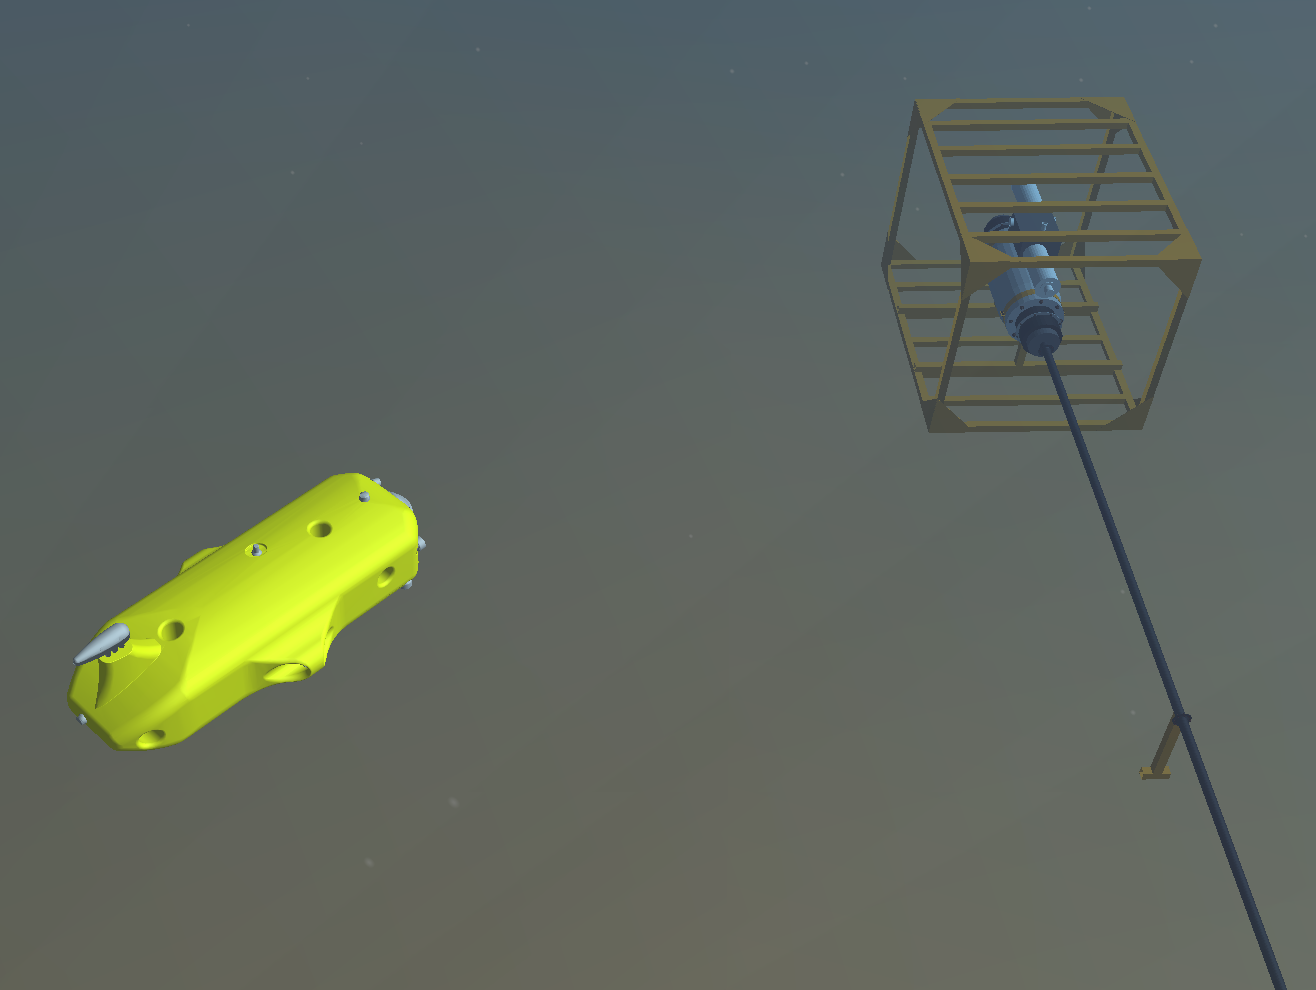
\includegraphics[width=0.425\paperwidth,height=6cm]{figs/fls_scene3}
        \label{fig:fls_scene3}
    }
    \subfigure[][]{
        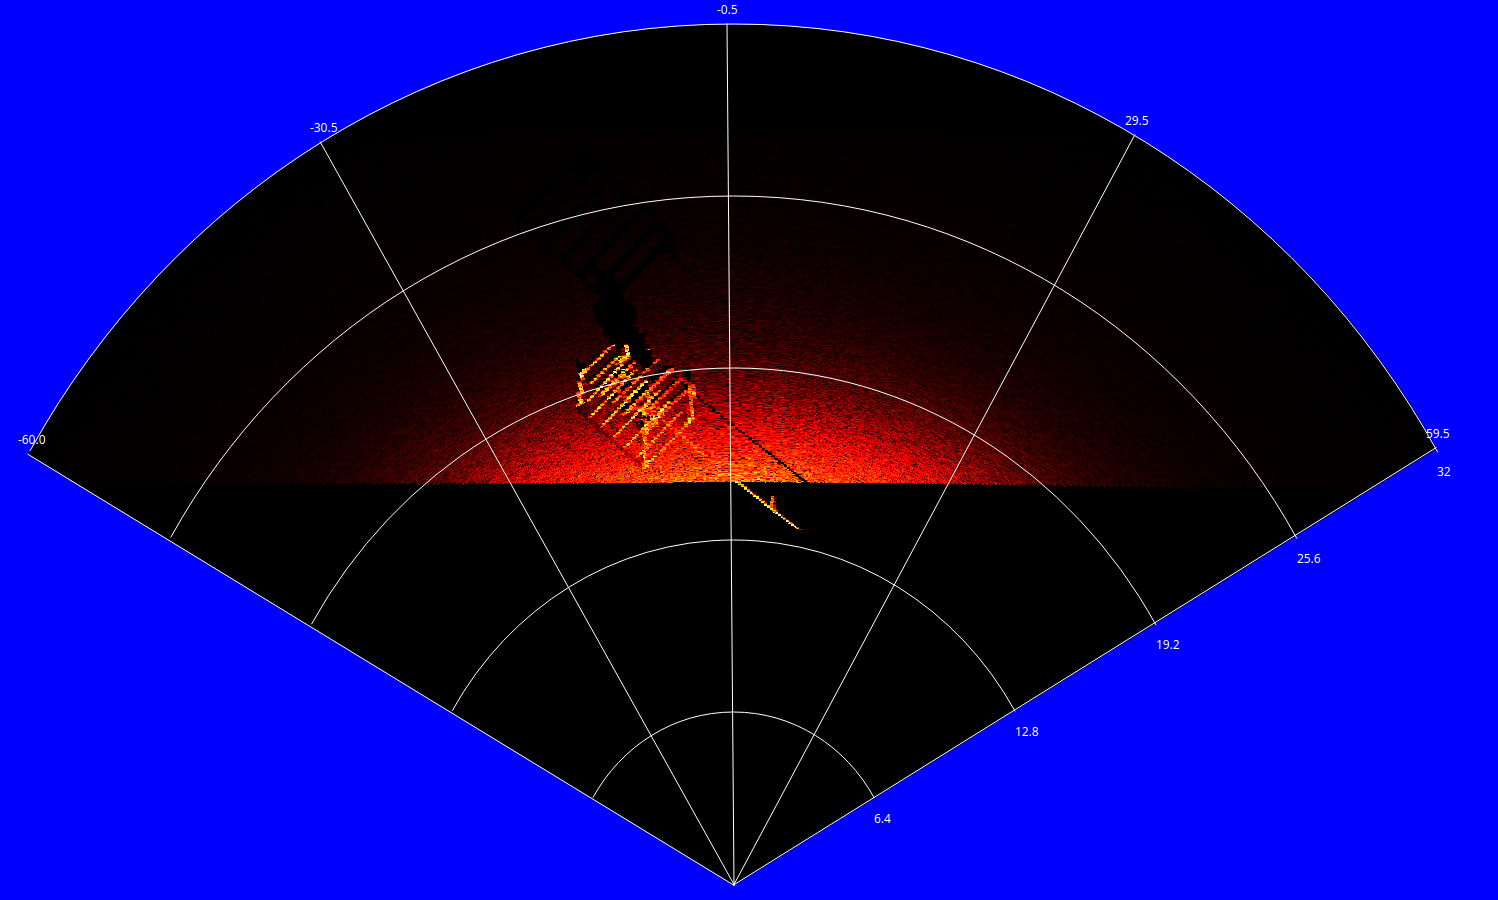
\includegraphics[width=0.425\paperwidth,height=6cm]{figs/fls_sim3}
        \label{fig:fls_sim3}
    }
    \captionsetup{justification=centering}
    \caption{Forward-looking sonar simulation experiments: Figs. \subref{fig:fls_scene1}, \subref{fig:fls_scene2} and \subref{fig:fls_scene3} presents the trials underwater scenarios and Figs. \subref{fig:fls_sim1}, \subref{fig:fls_sim2} and \subref{fig:fls_sim3} are the following acoustic representations, respectively.}
    \label{fig:fls}
\end{figure*}

The MSIS sensor was also simulated in three different experiments. The FlatFish robot in a big textured tank composed the first scene, as seen in Fig. \ref{fig:msis_scene1}. Even as the first scenario of FLS experiment, the reflectivity and texture were set to the target. The rotation of frontal sonar head position, by a complete $360^{\circ}$ scanning, produced the acoustic frame of tank walls, seen in Fig. \ref{fig:msis_sim1}.

The second experiment involves the vehicle's movement during the data acquisition process. The scene contains a grid around the AUV, as seen in Fig. \ref{fig:msis_scene2}, and the frontal MSIS is used. This trial induces a distortion in the final acoustic frame, because the relative sensor's position with respect to surrounding object changes while the sonar image is being built, as seen in Fig. \ref{fig:msis_sim2}. In this case, the robot rotates $20^{\circ}$ left during the scanning.

The last scenario presents the AUV over oil and gas structures on the sea bottom, as seen in Fig. \ref{fig:msis_scene3}. Using the back MSIS, with a vertical orientation, the scene was scanned in order to produce the acoustic visualization. As seen in Fig. \ref{fig:msis_sim3}, the objects' surfaces present clear definition in the small scanning section of the seafloor.

\begin{figure*}[!h]
    \centering
    \subfigure[][]{
        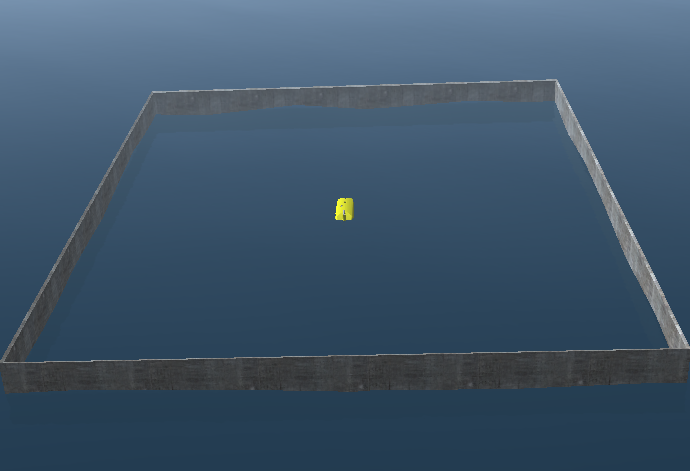
\includegraphics[width=0.425\paperwidth,height=6cm]{figs/msis_scene1}
        \label{fig:msis_scene1}
    }
    \subfigure[][]{
        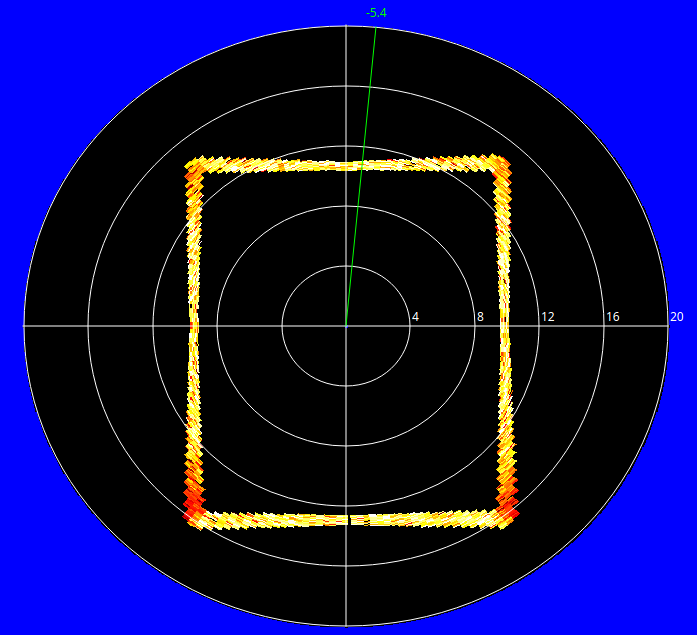
\includegraphics[width=0.425\paperwidth,height=6cm]{figs/msis_sim1}
        \label{fig:msis_sim1}
    }
    \subfigure[][]{
        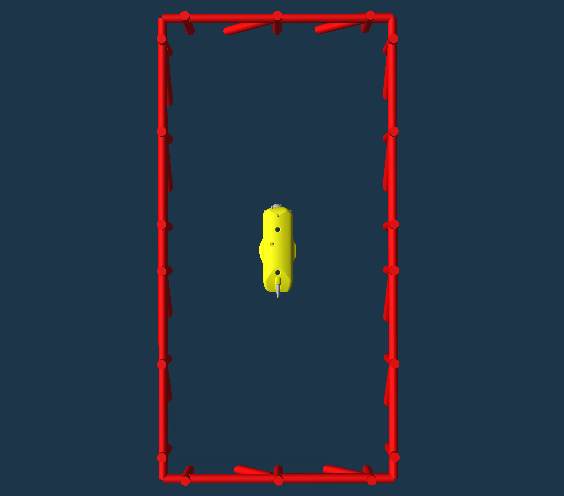
\includegraphics[width=0.425\paperwidth,height=6cm]{figs/msis_scene2}
        \label{fig:msis_scene2}
    }
    \subfigure[][]{
        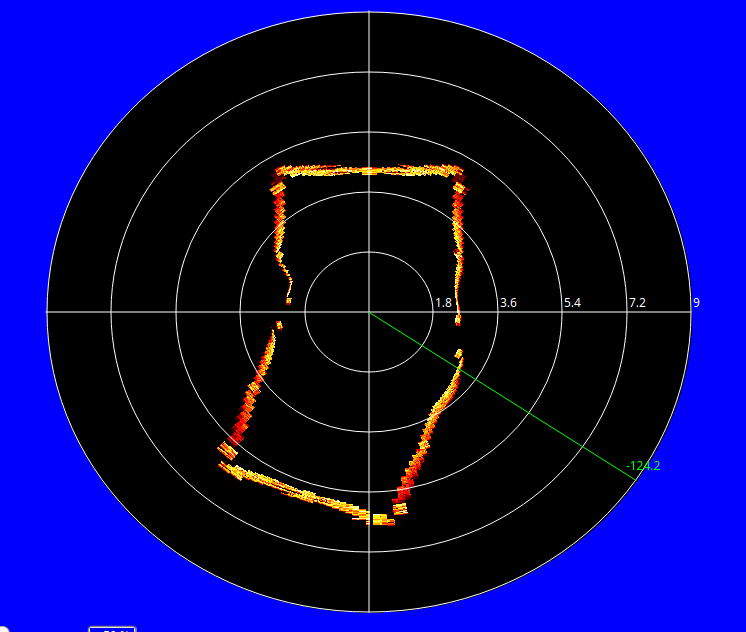
\includegraphics[width=0.425\paperwidth,height=6cm]{figs/msis_sim2}
        \label{fig:msis_sim2}
    }
    \subfigure[][]{
        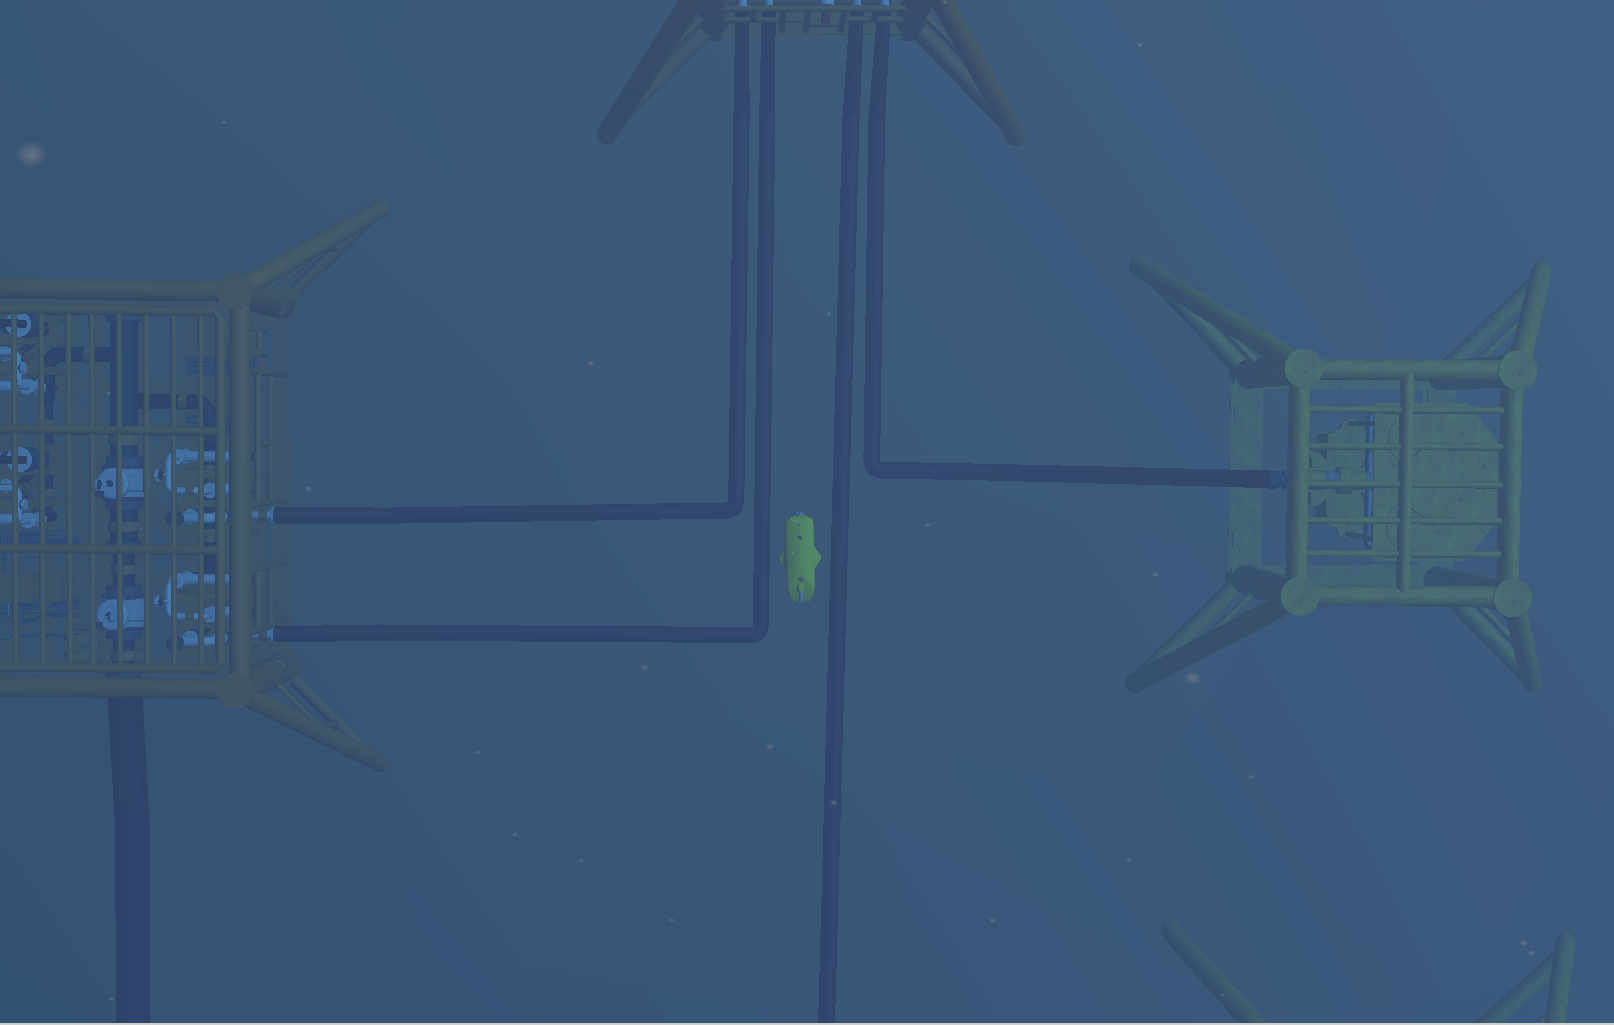
\includegraphics[width=0.425\paperwidth,height=6cm]{figs/msis_scene3}
        \label{fig:msis_scene3}
    }
    \subfigure[][]{
        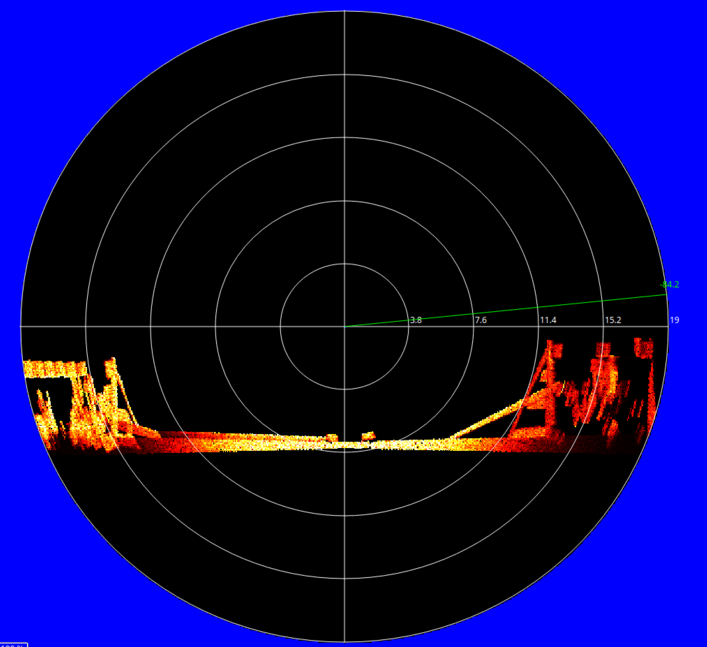
\includegraphics[width=0.425\paperwidth,height=6cm]{figs/msis_sim3}
        \label{fig:msis_sim3}
    }
    \captionsetup{justification=centering}
    \caption{Mechanical Scanning Imaging Sonar trials: the underwater scenes represented in Figs. \subref{fig:msis_scene1}, \subref{fig:msis_scene2} and \subref{fig:msis_scene3} and their following simulated frames in Figs. \subref{fig:msis_sim1}, \subref{fig:msis_sim2} and \subref{fig:msis_sim3}.}
    \label{fig:msis}
\end{figure*}

% The different scenarios here provided sufficient variability to detect several features found in real sonar images.

\subsection{Computation time}

The performance evaluation for this approach was determined as part of suitable analysis for real-time applications. The experiments were performed on a personal computer with Ubuntu 16.04 64 bits, Intel Core i7 3540M processor running at 3 GHz with 16GB DDR3 RAM memory and NVIDIA GF108GLM video card.

The elapsed time of each sonar data is stored to compute the mean and standard deviation metrics, after $500$ iterations, as presented in Tables \ref{table:fls} and \ref{table:msis}. After changing the device parameters, such as number of bins, number of beams and field of view, the proposed approach generated the sonar frames with a high frame rate, for both sonar types. Given the Tritech Gemini 720i, a real forward-looking sonar sensor with a field of view of $120^{\circ}$ by $20^{\circ}$ and 256 beams presents a maximum update rate of 15 frames per second, the results grant the usage of the sonar simulator for real-time applications. Also, the MSIS data built by the simulator is able to complete a $360^{\circ}$ scan sufficiently time short in comparison with a real sonar as Tritech Micron DST.

Moreover, since the number of bins is directly proportional to sonar image resolution, as explained in Section \ref{dev:sonardata}, this is also correlated with the computation time. When the number of bins increases, the simulator will have a bigger scene frame to compute and generate the sonar data.

\begin{table*}[!h]
    \caption{Processing time to generate FLS frames with different parameters.}
    \label{table:fls}
    \begin{center}
        \begin{tabular}{| c | c | c | c | c |}
            \hline
            Number of Beams & Number of Bins & Field of View & Mean ($sec$) & Standard Deviation ($sec$) \\
            \hline
            128     & 500       & $120^{\circ}$ x $20^{\circ}$        & 0.0546834   & 0.00373812  \\ \hline
            128     & 1000      & $120^{\circ}$ x $20^{\circ}$        & 0.0722763	& 0.00894485  \\ \hline
            256     & 500       & $120^{\circ}$ x $20^{\circ}$        & 0.19877	    & 0.0170872   \\ \hline
            256     & 1000      & $120^{\circ}$ x $20^{\circ}$        & 0.218282	& 0.0119873   \\ \hline
            128     & 500       & $90^{\circ}$ x $15^{\circ}$         & 0.0774186	& 0.0118534   \\ \hline
            128     & 1000      & $90^{\circ}$ x $15^{\circ}$         & 0.0945958	& 0.0102294   \\ \hline
            256     & 500       & $90^{\circ}$ x $15^{\circ}$         & 0.260864	& 0.0184956   \\ \hline
            256     & 1000      & $90^{\circ}$ x $15^{\circ}$         & 0.26867	    & 0.0166807   \\ \hline
        \end{tabular}
    \end{center}
\end{table*}

\begin{table*}
    \caption{Processing time to generate MSIS samples with different parameters.}
    \label{table:msis}
    \begin{center}
        \begin{tabular}{| c | c | c | c |}
            \hline
            Number of Bins & Field of View & Mean ($sec$) & Standard Deviation ($sec$) \\
            \hline
            500       & $3^{\circ}$ x $35^{\circ}$        & 0.00881959	& 0.000709754  \\ \hline
            1000      & $3^{\circ}$ x $35^{\circ}$        & 0.0345122	& 0.0015794    \\ \hline
            500       & $2^{\circ}$ x $20^{\circ}$        & 0.0103457	& 0.000665683  \\ \hline
            1000      & $2^{\circ}$ x $20^{\circ}$        & 0.0417138	& 0.00368668   \\ \hline
        \end{tabular}
    \end{center}
\end{table*}

% ----------------------------------------------------------------------------------

\section{Conclusion and Outlook}
\label{conclusion}

We presented a GPU-based approach for imaging sonar simulation. By the evaluation results on different scenarios, the targets were well-defined on simulated sonar frames. The same model was able to reproduce the sensoring of two kind of sonar devices (FLS and MSIS). Moreover, the real sonar image singularities, such as speckle noise, surface irregularities, shadows, material properties and shapes are also addressed and represented on the synthetic acoustic images.

In addition, the processing time was calculated with different sonar parameters (field of view, number of bins and number of beams). The vertex and fragment processing during the underwater scene rendering accelerates the sonar image building and the mean and standard deviation metrics certified the performance is much closely to real imaging sonars. Therefore, the results granted the usage of this imaging sonar simulator by real-time applications, such as target tracking, obstacle avoidance and localization and mapping algorithms.

Next steps will focus on qualitative and computation-efficiency evaluations with other imaging sonar simulators.

%% The Appendices part is started with the command \appendix;
%% appendix sections are then done as normal sections
%% \appendix

%% \section{}
%% \label{}

%% References
%%
%% Following citation commands can be used in the body text:
%% Usage of \cite is as follows:
%%   \cite{key}          ==>>  [#]
%%   \cite[chap. 2]{key} ==>>  [#, chap. 2]
%%   \citet{key}         ==>>  Author [#]

\section*{Acknowledgment}
%
The authors would like to thank Shell Brazil and ANP for financing the work and SENAI CIMATEC and DFKI RIC for the great institutional support.

%% References with bibTeX database:
% \newpage

% \nocite{*}
\bibliographystyle{model3-num-names}
\bibliography{elsarticle-template-3-num}

%% Authors are advised to submit their bibtex database files. They are
%% requested to list a bibtex style file in the manuscript if they do
%% not want to use model3-num-names.bst.

%% References without bibTeX database:

% \begin{thebibliography}{00}

%% \bibitem must have the following form:
%%   \bibitem{key}...
%%

% \bibitem{}

% \end{thebibliography}


\end{document}

%%
%% End of file `elsarticle-template-3-num.tex'.
